% Chapter Template
\chapter{Analysis} % Main chapter title

\label{Chapter4} % Change X to a consecutive number; for referencing this chapter elsewhere, use \ref{ChapterX}

\section{Data Summary} \label{Data Summary}

After parsing and cleaning the data is stored in two tables, a patent table and a citation table as shown in tables \ref{tab:patents} and \ref{tab:citations}. Definitions of variables are described in section \ref{section:Cleaning}.

The dataset covers the time period from 1976 to 2015, over this period 5,803,302 patents have been processed along with 114,585,378 citations. Since 2001 where the data dictating who cited each citation was initially released 25.7\% of citations have been the Examiner and the rest being other sources. Since 2005 where accurate country codes for foreign patents have been released 85.5\% of citations have been internal, i.e. to other US patents.

\begin{table}[ht]
\caption{First 6 entries in parsed and cleaned patent table, 1976}
\label{tab:patents}
\centering
\begin{tabular}{rlrrr}
  \hline
 & Patent & Date & Order & Date2 \\ 
  \hline
  1 & RE28671 & 19760106 &   8 & 2196 \\ 
  2 & RE28672 & 19760106 &   7 & 2196 \\ 
  3 & RE28673 & 19760106 &   3 & 2196 \\ 
  4 & RE28674 & 19760106 &   5 & 2196 \\ 
  5 & RE28675 & 19760106 &  13 & 2196 \\ 
  6 & 3930271 & 19760106 &   2 & 2196 \\ 
   \hline
\end{tabular}
\end{table}

\begin{table}[ht]
\caption{First 6 entries in parsed and cleaned citation table}
\label{tab:citations}
\centering
\begin{tabular}{rllrllr}
  \hline
 & Patent & Citation & Date & CitedBy & Country & Date2 \\ 
  \hline
1 & D607176 & 534632 & 18950200 & cited by examiner & US & -27362 \\ 
  2 & D607176 & D28957 & 18980600 & cited by other & US & -26146 \\ 
  3 & D607176 & D45899 & 19140600 & cited by other & US & -20303 \\ 
  4 & D607176 & D59909 & 19211200 & cited by examiner & US & -17563 \\ 
  5 & D607176 & D96223 & 19350700 & cited by examiner & US & -12603 \\ 
  6 & D607176 & D96224 & 19350700 & cited by examiner & US & -12603 \\ 
   \hline
\end{tabular}
\end{table} 
%----------------------------------------------------------------------------------------
%	SECTION 1: Patents per Year
%----------------------------------------------------------------------------------------
\section{Network Summary} \label{Network Summary}

In this section some general summaries of the network are computed. Some of these summaries have been previously carried out by other authors allowing validation of this/their analysis. 

%-----------------------------------
%	SUBSECTION 1: Cumulative distribution 
%-----------------------------------

\subsection{Patents per Year} \label{Patents per Year}

\begin{figure}
\centering
 \centering
 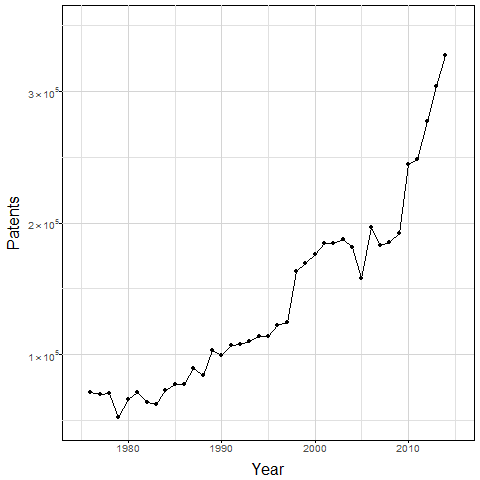
\includegraphics[width=0.7\linewidth]{Figures/PatentCountVsYear}
\caption[Number of patents granted each year]{Number of patents granted each year from 1976 to 2014}
\label{fig:PatentCountVsYear}
\end{figure}

Each patent was grouped by the year in which it was published and frequency computed. The year 2015 was omitted due to the presence of two missing months of data due to a download error on the part of the USPTO as discussed in the previous section. 

Figure \ref{fig:PatentCountVsYear} shows the number of patents granted each year on linear scales. There are two main features: a large jump between 1997 and 1998 and a transition to very rapid growth after 2009. Note that these events don't align themselves with changes in the data format which occur from 2001-2002 and from 2004-2005. This transition may be caused by socio-economic or political effects as it occurs directly after the 2008 recession, regardless the continued growth after 2009 indicates a change in the evolution of the network. Valverde et al. \cite{valverde2007topology} conducts a similar analysis, over the years of 1986 to 2005, which has the same general shape but some minor differences; most visibly in the size of the gap between 1997 and 1998 which is bigger in this analysis than the former. In the previous chapter patent counts per year were compared to other sources, USPTO summary statistics and the 'lst' files, consistency of these points to some possible difference in methodology or parsing errors in the case of Valverde's paper. 

Valverde et al. claims that this metric of patents granted per year follows a power law distribution. To demonstrate this they plot the cumulative number of patents on log-log scales and make a linear fit. To replicate this analysis patent counts per year the cumulative number of patents in the network is computed and plotted on logarithmic scales. A generalised linear model is fitted using least squares regression and a log-log transform. 

Figure \ref{fig:CumPatents2} shows the cumulative number of patents granted over time starting in 1976 and ending in 2014. Time is given as number of years from the origin. Figure (A) shows a power-law model fitted to the entire dataset and its exponent whereas figure (B) conducts this method only on the years 1986 to 2005. The cumulative distribution is often used to identify power-law behaviour because often the tail of the distribution has rare events with large amounts of statistical noise, the cumulative integrates the noise into a smooth function. If $ p(x) = x^{\alpha}$ the cumulative distribution is also a power law with smaller exponent:

$$ P(x) =  \frac{1}{\alpha - 1}x^{(\alpha - 1)}$$

While not necessary in this instance due to the absence of a noisy tail, a CDF was used to closely replicate the Valverde methodology and is general best practice. Although using least squares regression on a log-log transformed cumulative distribution is not the most rigorous method for fitting power-law distributions introducing small bias to the exponent, this appears to be the methodology used in the Valverde paper (although it is not clear) additionally the exact value of the exponent is not important only the general shape of the model. 


\begin{figure}
\centering
\begin{subfigure}{.5\textwidth}
  \centering
  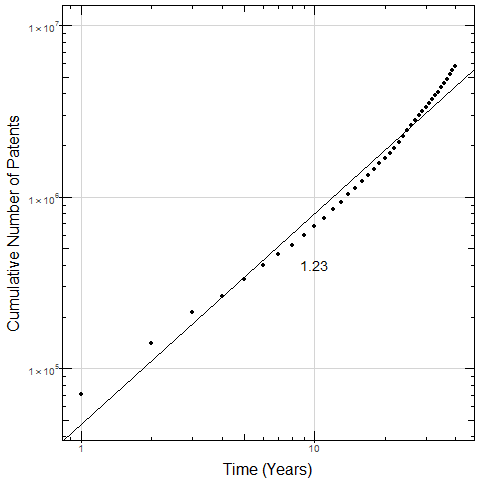
\includegraphics[width=0.7\linewidth]{Figures/CumulativePatents1}
 \caption[CumPatents1]{\small}
\label{fig:CumPatents1}
\end{subfigure}%
\begin{subfigure}{.5\textwidth}
  \centering
  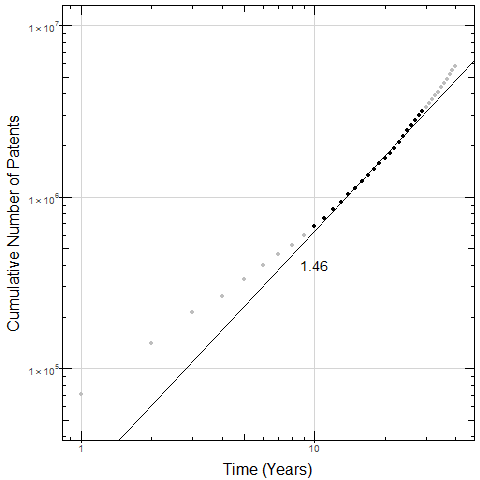
\includegraphics[width=0.7\linewidth]{Figures/CumulativePatents2}
  \caption[CumPatents1]{\small G}
\label{fig:CumPatents2}
\end{subfigure}
\caption[Power-law fit for cumulative number of patents granted each year]{The cumulative number of patents granted from 1976 to 2015, plotted on a log-log scales. Fitted with generalised linear model of the form $y = x^{\alpha}$ using (A) all the data and (B) only the data in over the years 1986 to 2005.}
\label{fig:CumPatents}
\end{figure}

From \ref{fig:CumPatents1} there is a clear divergence from the fit over the first few years. In Valverde's paper it appears that in their paper they may have disregarded these first few points as outliers, this can be shown by figure \ref{fig:CumPatents2} which omits these points yielding a very similar exponent (1.46 vs. 1.45). Since 2005 where their data-set ended new data-points do not fit this model well. This is more apparent in figure \ref{fig:patentCountFit} which shows this same fit on the non-cumulative plot. 

Using the same methodology as before an exponential fit to the data is produced, \ref{tab:distributions}. This is shown on figure \ref{fig:cumulativePatentFits} with a 95\% confidence interval along side the original power-law fit. 

\begin{figure}
\centering
\begin{subfigure}{.3\linewidth}
  \centering
  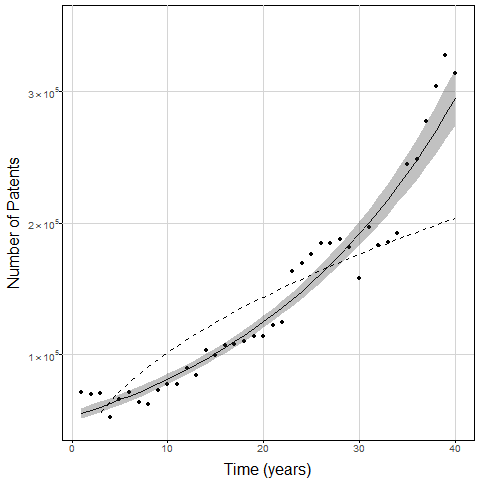
\includegraphics[width=0.9\linewidth]{Figures/patentCountFit}
 \caption[CumPatents1]{\footnotesize Patents granted per year}
\label{fig:patentCountFit}
\end{subfigure}%
\begin{subfigure}{.3\linewidth}
  \centering
  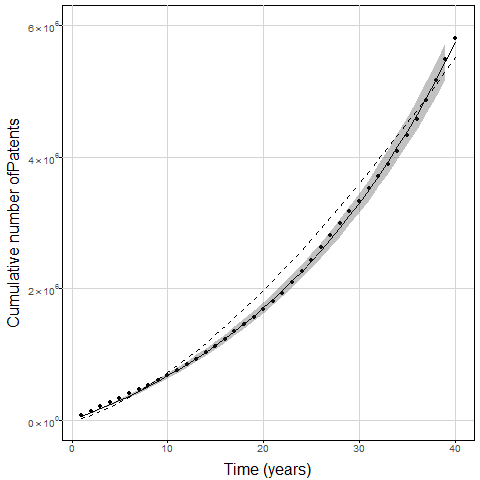
\includegraphics[width=0.9\linewidth]{Figures/patentCountFit_cum}
  \caption[CumPatents1]{\footnotesize Cumulative number of patents granted}
\label{fig:patentCountFit_cum}
\end{subfigure}
\begin{subfigure}{.3\linewidth}
  \centering
  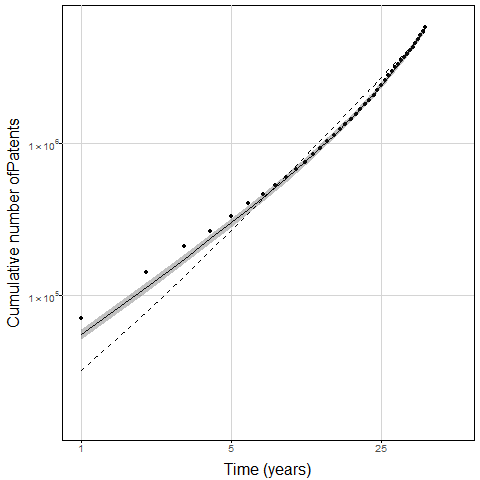
\includegraphics[width=0.9\linewidth]{Figures/patentCountFit_cum_loglog}
  \caption[CumPatents1]{\footnotesize Cumulative patents granted on a log-log scale}
\label{fig:patentCountFit_cum_loglog}
\end{subfigure}
\caption[Exponential fit for number of patents granted each year]{Power law and exponential fits for cumulative number of patents published each year}
\label{fig:cumulativePatentFits}
\end{figure}

It is clear that a power-law fit doesn't fit the data, it is plausible that an exponential model may be more accurate (fig.\ref{fig:cumulativePatentFits}). However the presence of two major shifts in the distribution in 1997/8 and 2009/10 indicate that large external effects are causing changes in this data-set. These changes are significant enough that without taking them into account or aggregating over a longer period of time or smaller timescales making a statistically significant claim about the underlying distribution here would be difficult.  

%-----------------------------------
%	SUBSECTION 1: Cumulative distribution 
%-----------------------------------


\subsection{Degree Distribution} \label{Degree Distribution}

The degree distribution is the frequency distribution of patents with respect to the total number of citations they make. It can inform how new citations are made and copes well with the evolution of the network over time as analysing years separately they do not need to be normalised. This has been separated into different years and the years 1984,1992, 2002 and 2012 have been on a log-log scale and fitted with a generalised linear model as before to replicate the third plot in the Valverde paper \ref{fig:OrderDistribution}. 

The exponent of the power-law is increasing over time, indicating both more citations over time but more extreme values also. These values however are quite different from those found by Valverde who found an exponent of -4.0 in 2002. This may be due to a number of methodology differences, most likely that our analysis includes foreign patents. We see that the frequency increases to a peak giving the distributions a mode of 6 to 8 depending on year, after around 10 to 20 this appears to converge to a power law.

\begin{figure}
\centering
  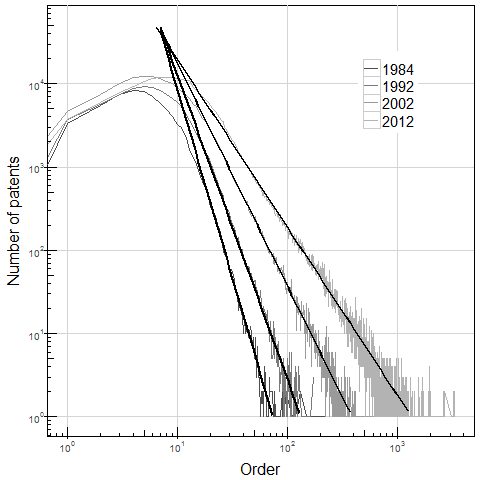
\includegraphics[width=0.7\linewidth]{Figures/OrderDistribution}
  \caption[Degree Distribution]{Degree distribution (number of citations for each patent) on a log-log scale shown for years 1984,1992,2002,2012. Fit with generalized linear model of the form $y \sim x^\alpha$ yielding exponents of minus 6.31, 6.92, 7.77 and 8.46 respectively}
\label{fig:OrderDistribution}
\end{figure}

As before some best practices have been ignored in order to reproduce the Valverde et al. paper better. Valverde claims that this distribution follows an extended power law of the form $ P(k) \sim (k + k_0)^{-\gamma} $, where $k$ is the degree and $k_0$ and $\gamma$ are constants. An extended power-law  converges to a power law of $k >> k_0$ and converges to an exponential for $ k << k_0$, it is therefore functionally similar to the popular model of a power-law with an exponential cut-off. They do not however state how they make their fit or conduct any tests to identify the efficacy of such a fit. 

Considering the 4 different years presented in figure \ref{fig:OrderDistribution} and the 4 most popular discrete distributions described in table \ref{tab:distributionsP}, each of these functional forms is fitted to the cumulative frequency order distribution by maximising their likelihood functions. The cumulative distribution is used as it mitigates noise caused by low frequency events. This is done while optimising the cut-off value $x_{min}$ for that distribution. Optimising $x_{min}$ uses a method proposed by Clauset et al. which searches over a range of values and minimises the difference in probability distributions of the data and the fit \cite{clauset2007frequency}. The difference metric used is the Kolmogorov-Smirnov statistic; the maximum distance between the two distributions. 

The accuracy of these fits is assessed using a bootstrapping algorithm, the distribution is sampled with replacement $n$ times, each time the KS statistic is computed between this sampled distribution and the original data. The P value is given as the proportion of sample distributions less similar to the original distribution than the fit. A rule of thumb given by Clauset et al. states to achieve an error of approximately $\epsilon$ the number of samples used should be at least $\frac{1}{4}\epsilon^{-2}$. 2500 samples were used to achieve $\epsilon \approx 0.01$ \cite{clauset2009power}. 

From figure \ref{fig:distributionFits} we see the increasing gradient of the power-law exponent over time, additionally the distribution appears to become less straight and has greater changes in shape at the tail, which was harder to identify using the non-cumulative plot \ref{fig:OrderDistribution}. As the distribution becomes less straight the power-law fit becomes less accurate especially failing to capture the shape of the tail. The Poisson and exponential distribution never successfully fit the main body of the data, the Poisson distribution especially fails in this regard fitting either poorly in 1984 or to increasingly small subsections of the tail in later years. The exponential function follows a similar trend, fitting the main body of the data poorly initially before trying to fit only the tail of the distribution, matching the exponential with the power-law suggests that an exponential cut-off is plausible however the log-normal distribution also appears to be a good fit, capturing some of the behaviour of the tail in a way none of the other distributions were able to. 

\begin{table}
\caption{Functional form and maximum likelihood estimate (MLE) of distributions tested}
\label{tab:distributions}
\centering
\begin{tabular}{l l l}
\toprule
Distribution & $f(x)$ & MLE\\
\midrule
Power Law & $ x^{-\alpha}$ & $ \hat{\alpha} = 1 + n[\sum^n_{i=1}ln\frac{x_i}{x_{min}}]^{-1} $ \\
Log-Normal & $\frac{1}{x}exp[-\frac{(lnx-\mu)^2}{2\sigma^2}] $  & $ \hat{\mu} = \frac{\sum lnx}{n}, \hat{\sigma^2} = \frac{\sum_k(lnx_k - \mu)^2}{n} $ \\
Exponential & $ \exp^{-\lambda x}$  & $\hat{\lambda} = \frac{1}{\bar{x}} $ \\
Poisson & $ \frac{\lambda^x\exp^{-\lambda}}{x!}$ & $\hat{\lambda} = {\sum^n_{i=1}k_i}{n} $ \\ 
\bottomrule\\
\end{tabular}
\end{table}

\begin{figure}
\centering
  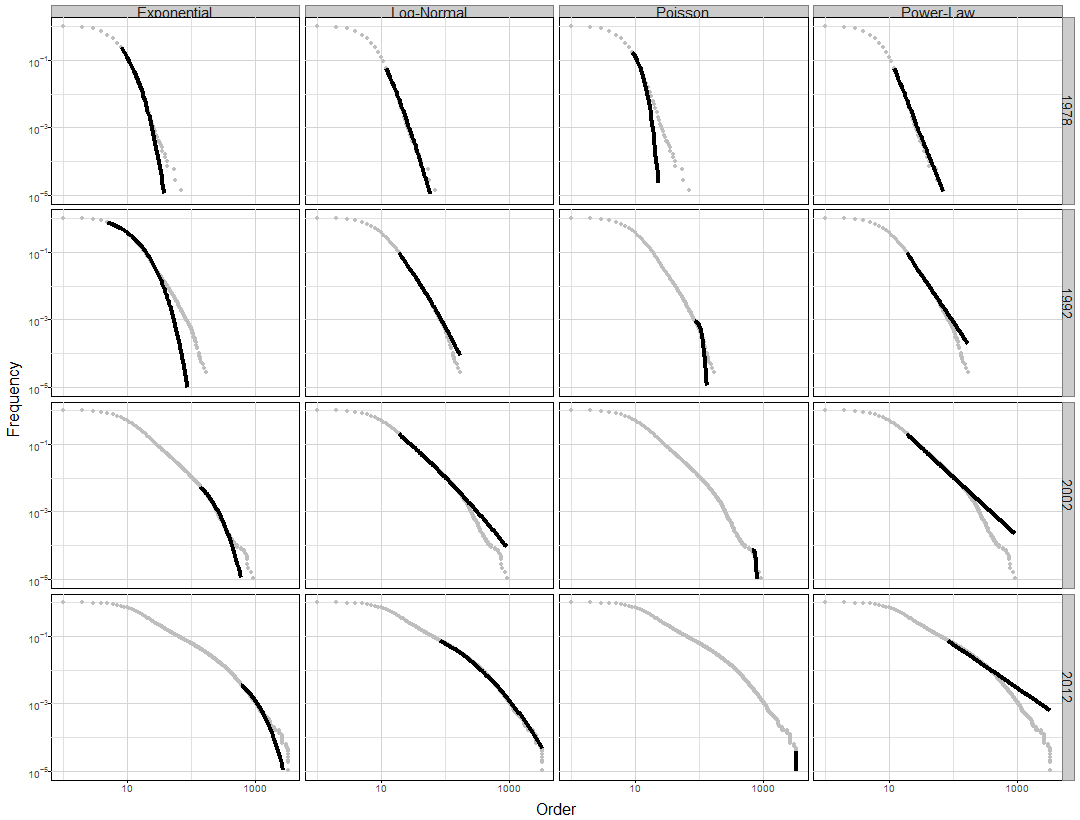
\includegraphics[width=\linewidth]{Figures/distributionFits}
  \caption[]{Cumulative density function fitted using maximum likelihood estimates for Poisson, Exponential, Log-normal and Power-law distributions}
\label{fig:distributionFits}
\end{figure}

\begin{table}
\caption{P values fitting distributions to the degree distribution obtained through bootstrapping method on a n = 10000 sample of the data}
\label{tab:distributionsP}
\centering
\begin{tabular}{l l l l l}
\toprule
Year & Power-Law & Log-Normal & Poisson & Exponential \\
\midrule
1984 & 0.494 & 0.302 & 0.000 & 0.001 \\
1992 & 0.820 & 0.934 & 0.000 & 0.005 \\
2002 & 0.534 & 0.399 & 0.108 & 0.000 \\
2012 & 0.266 & 0.280 & 0.000 & 0.448 \\
\bottomrule\\
\end{tabular}
\end{table}

Note that this bootstrapping procedure is conducted on a sample of 1000 observations due to heavy performance issues with the algorithm while the distribution fits use the entire dataset, this can lead to large differences between the two as different $x_{min}$ values are optimised. For example in 2002 and 2012 the Poisson distribution has a very large $x_{min}$ and therefore a higher p value would be expected than when it poorly fits to the whole curve. While the small sample size relative to the size of the data may limit the insight from this test, the consistently low and often 0 values of the Poisson and Exponential distributions means they can likely be dismissed as candidates for this distribution. 

While the power-law and log-normal distributions are consistently significant it is not sufficient to say that the power-law is better than the log-normal. To compare the models directly Vuong's test is used \cite{vuong1989likelihood}, this is based on the null hypothesis that both fits are equally far from the true distribution, if true the log-likelihood is expected to have a Normal distribution. This test is done using the complete data (without sampling) using the fits shown in figure \ref{fig:cumulativePatentFits}. 

\begin{table}
\caption{P values giving upper limit of if power-law is true (one-sided) or both power-law and log-normal distributions are equally good (two-sided) using Vuong's test}
\label{tab:Vuong}
\centering
\begin{tabular}{l l l}
\toprule
Year & One-sided & Two-sided \\
\midrule
1984 & 3.87e-1 & 7.74e-1  \\
1992 & 1.39e-4 & 2.78e-4  \\
2002 & 1.1e-10 & 2.3e-10  \\
2012 & 9.3e-86 & 1.9e-85  \\
\bottomrule\\
\end{tabular}
\end{table}

The power law is never the more likely distribution based on this test but in 1984 it is significant to the degree that the two-sided test, indicating both distributions are equally likely has high p-value. However this likelihood of a power law being true consistently decreases over time so that in 2012 there is a $9.3 \times 10^{-86}$ chance of a power-law in contrast to the log-normal distribution. 

%----------------------------------------------------------------------------------------
%	SECTION 1
%----------------------------------------------------------------------------------------

\section{Coloured Network Analysis} \label{Coloured Network Analysis}

One of the features parsed was who contributed the citation to the patent document. From 2001 to 2013 this is split into two categories "Cited by Examiner" and "Cited by Other". The Examiner has a duty to fulfil the legal requirements of the patent application citing any prior art which was absent from the patent previously. Cited by Other "indicates those cited in a protest, by an attorney or agent not acting in a representative capacity but on behalf of a single inventor, and by the applicant" \cite{USPTOSummary}. In reality all sources of citation besides the applicant are rate, this is shown in 2014 and 2015 where the 'cited by other' field was split into two, 'cited by applicant' and 'cited by third party'. Over these two years 99.999\% of these citations were 'cited by applicant' rather than the third party. For the sake of consistent analysis these have been combined again into a 'cited by other' category.

This 'citedBy' field was analysed because of the differing motivations and responsibilities of the parties involved. The Examiner with a legal and professional responsibility is likely to act differently from the applicant and many of the features that make the patent network unique are the legal responsibilities that citations have so studying this sub-network could yield more varied results than the network as a whole, especially when compared to other bibliographic networks. 

\subsection{Degree Distribution}
The degree distribution of for the two sub-networks are calculated in the same way as section \ref{Degree Distribution} shown in figure \ref{fig:orderDistributionCitedBy} and the mean degree for each of the two sub-networks and total are calculated for each year \ref{fig:av_degree_vs_year}.

\begin{figure}
\centering
\begin{subfigure}{\textwidth}
  \centering
  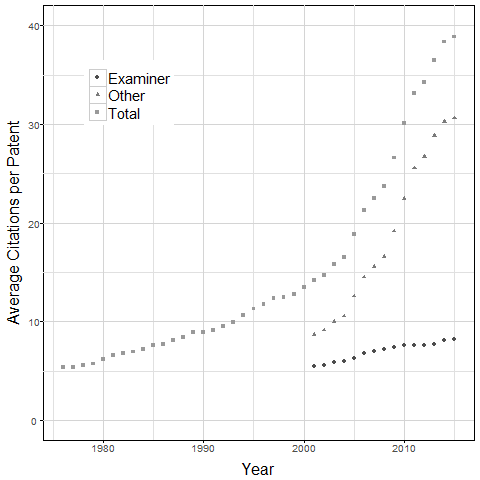
\includegraphics[width=0.7\linewidth]{Figures/av_degree_vs_year}
 \caption[]{\small Average degree by citedBy for the years 2001 to 2015 and average total degree from 1976 to 2015}
\label{fig:av_degree_vs_year}
\end{subfigure}%

\begin{subfigure}{\textwidth}
  \centering
  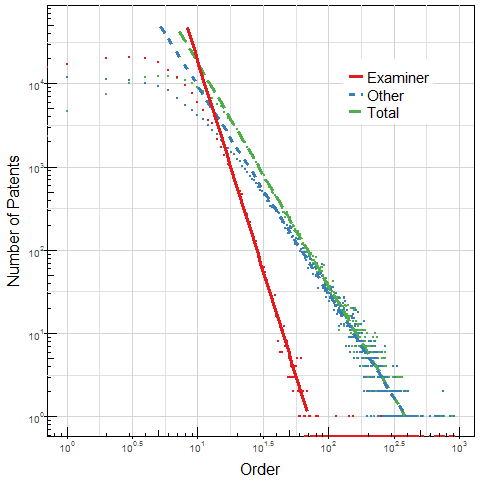
\includegraphics[width=0.7\linewidth]{Figures/orderDistributionCitedBy}
  \caption[]{\small Degree distribution by citedBy on a log-log scale, fitted with generalised linear model of the form $y \sim x^{-\alpha}$, here total refers only to the years 2001 to 2015}
\label{fig:orderDistributionCitedBy}
\end{subfigure}
\caption[]{}
\label{fig:degreeCitedBy}
\end{figure}

The average number of citations for each patent changes very little over time for the Examiners but increases rapidly over the available data range for 'Other'. As Other dominates the Examiner the total value follows this closely this means that the structure of the Examiner network is masked. It is unclear how this relationship held over the previous years, it may be that the two sources of citation had a more harmonious relationship in the past as over the period of time from 1976 to 200 the increase in average citation over time is fairly constant and similar to the increase in time of the Examiner network. 

The exponent for the degree distribution is more negative for the examiner indicating that it operates over a smaller range of values, reaching a maximum at approximates 100 rather than 1000. The Examiner distribution also appears to be a better fit in the tail of the distribution and has higher frequencies at low citation counts. 

All of these features of the Examiner network relative to the Other network are not unexpected as they indicate more conservative and consistent practices which would be fairly typical of a professional. The large range of values may suggest a tendency for the applicants to occasionally over-cite their patents to an extreme. 

The changes in average citation number being caused by differences only in the applicants activity could damage the idea that there is a structure of innovation itself over this time period because it suggests that the patents themselves aren't necessarily becoming more interdependent as an increase in average citations per patent otherwise suggests. However this doesn't discount the idea as the Examiner acts after the applicant so changes to the patents/innovations themselves could be accounted for by their actions alone although this is a less likely explanation. 

%----------------------------------------------------------------------------------------
%	SECTION 2
%----------------------------------------------------------------------------------------

\subsection{Correlation} \label{Correlation}

In order to investigate the relationship between the Examiner citations and Other citations a number of analyses of correlation between the order of each is measured (number of Examiner citations vs. number of Other citations for each patent). 

A scatter-plot of all patents from 2001 to 2015 was made using a log-log scale, comparing the number of citations made by Examiners to those made by Others, because these orders are discrete a uniform random noise of $\pm 0.5$, this expands the data to uniformly occupy the area which rounds to its discrete value. This allows the density to be seen more clearly. The scatter-plot is made with a sample of 100,000 observations and a linear fit is added using least square regression to represent the correlation between the two. 

To more clearly represent the density of the scatter-plot a contour density graph is built on a log-log scale using two-dimensional kernel density estimation. This evaluates a bivariate normal kernel over the log-log transformed data to produce a density estimate. This is done without the random uniform noise because the discrete density is well represented already. The bandwidth of the kernel for a data vector $x$ is the normal reference bandwidth given by equation \ref{eq:bandwidth} \cite[page 130]{venables2013modern}: 

\begin{align} \label{eq:bandwidth}
\begin{split}
a &= \frac{Q_3(x) - Q_1(x)}{1.34} \\
b &= \sqrt[]{\sigma_x} \\
bandwidth &= 4 \times 1.06 \times min(a,b) \times N_x^{-1/5} 
\end{split}
\end{align}

The mean and median of one class is computed for logarithmically binned intervals of the other class. I.e. for the set of observations with Examiner degree in the first interval the mean and standard deviation of the Other degree is calculated (figure \ref{fig:MeanOtherVsExaminer}) as well as median and interquartile range (figure \ref{fig:MedianOtherVsExaminer}). The median is computed because heavy tailed distributions can be biassed using the mean and standard deviation only represents error (when transformed to standard error) under the assumption of a normal distribution. 

Finally correlation metrics are computed with p-values using the fBasics R package \cite{fBasics}. Pearson correlation is computed non-parametrically using a bootstrapping procedure. As Pearson correlation is a measure of linear correlation between variables a log-log transformed version was also computed. Kendall's Tau and Spearman's rho are rank based measures so work on non-parametric data natively, this means that the rho and the tau are not measures of a linear relationship like the Pearson product-moment correlation. 

\begin{figure}
\centering
\begin{subfigure}{\textwidth}
  \centering
  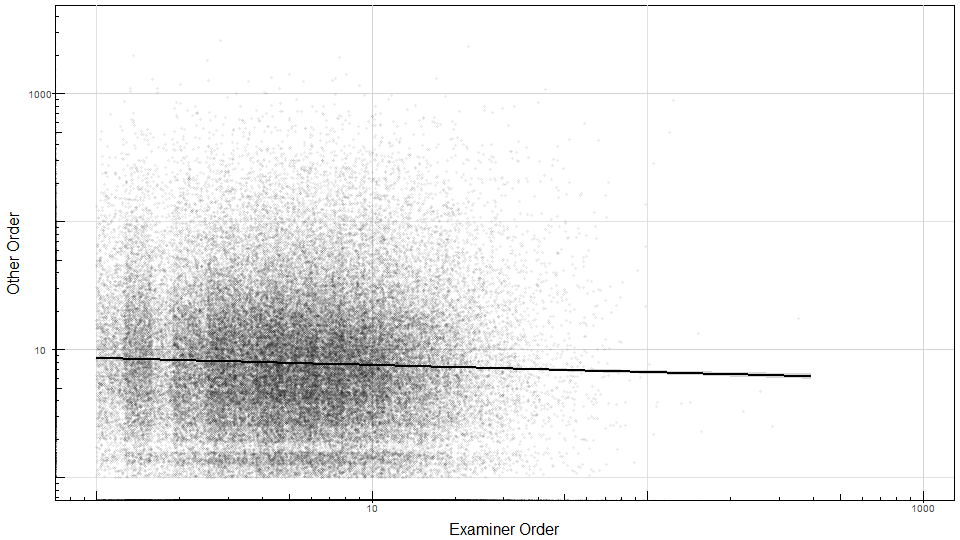
\includegraphics[width=0.9\linewidth]{Figures/orderScatterplot}
 \caption[]{\small Using log-log scale, linear fit shown \newline}
\label{fig:orderScatterplot}
\end{subfigure}%

\begin{subfigure}{\textwidth}
  \centering
  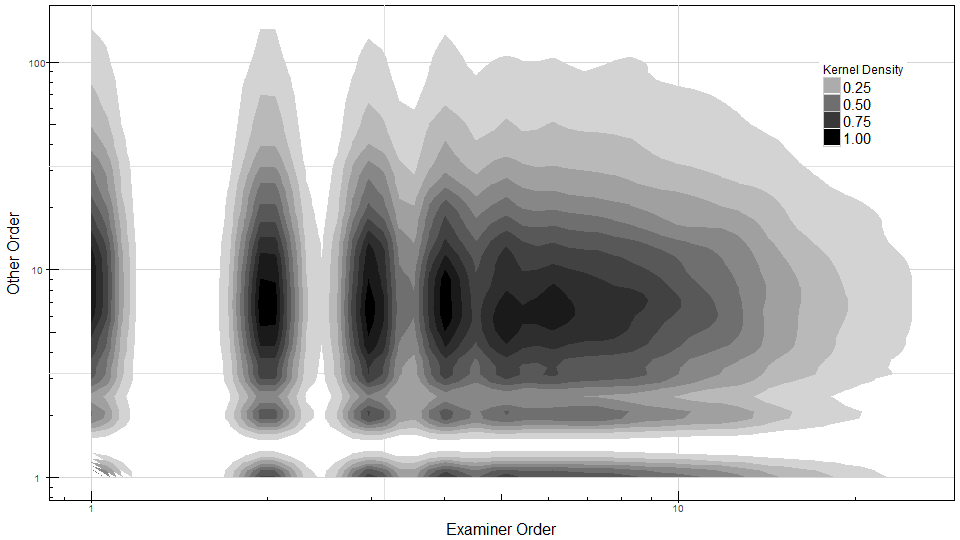
\includegraphics[width=0.9\linewidth]{Figures/orderScatterplotContours}
  \caption[]{\small Contour density graph using Kernel Density Estimator}
\label{fig:orderScatterplotContours}
\end{subfigure}
\caption[Scatterplot of Order for 'Other' and 'Examiner' sub-graphs]{Scatterplot of 'Examiner' and 'Other' orders for each patent using an n = 100,000 sample.}
\label{fig:scatterplots}
\end{figure}

In figures \ref{fig:orderScatterplot} and \ref{fig:orderScatterplotContours} it is clear that any correlation between the two orders are very small in nature, this is supported by all the correlation metrics computed (table \ref{tab:cor}). This is fairly unexpected, under a model that each patent has some underlying true number of citations and applicants have some fairly constant level of completeness for this true number that the correlation would be significant and positive as the greater true citation number the greater the number of citations from both examiner and applicant in this model. However under a model where the true number of citations is fairly constant but the distribution of completeness from the applicant varies a negative correlation would be expected because as the applicant finds most the relevant citations there are fewer left for the examiner to complete the patent. This model however assumes that both the examiner and the applicant are getting citations from a limited set of correct citations, if either is making a significant portion of their citations from outside this set then correlations would decrease. This is likely what is occurring either some of the parties are making citations from outside the set of correct citations and/or the set is not well defined. 

The data may support these models of correlation however, figure \ref{fig:MeanExaminerVsOther} shows a slight negative correlation for the bulk of the data but a positive correlation for the large order values and each of the correlation metrics are slightly negative. Figure \ref{fig:MeanExaminerVsOther} shows that extreme values have slightly positive correlation, while the error is large enough that this effect isn't statistically significant and the discrete nature of the median makes it difficult to identify trends in the other plots, the Kernal density plot does appear to corroborate this slight positive correlation for extreme orders. The Mean of the other for binned Examiner shows a similar effect but the positive correlation peaks before decreasing again, there are  very low sample sizes for these high values of Examiner. 

\begin{figure}
\centering
\begin{subfigure}{0.6\linewidth}
  \centering
  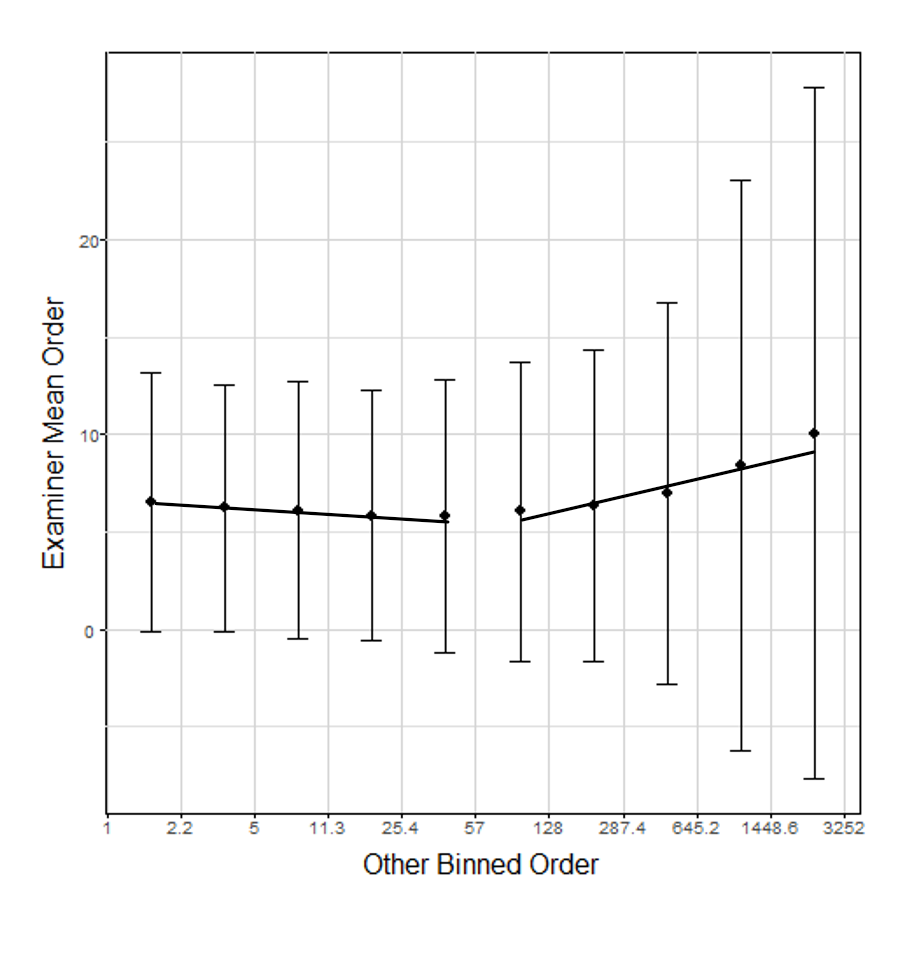
\includegraphics[width=0.9\linewidth]{Figures/MeanExaminerVsOther}
  \caption[]{\small Mean Examiner for Binned Other with two linear regressions over the first 5 bins and last 5 bins.}
\label{fig:MeanExaminerVsOther}
\end{subfigure}

\begin{subfigure}{.24\linewidth}
  \centering
  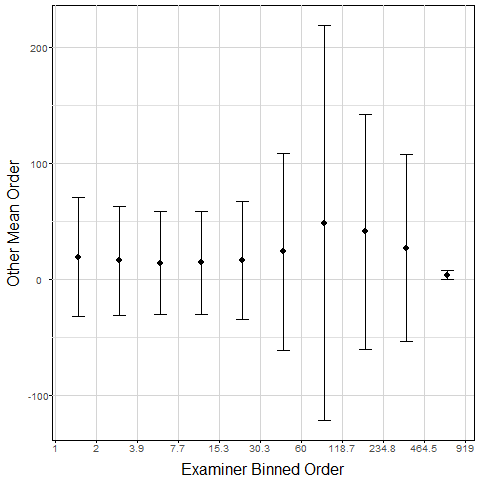
\includegraphics[width=0.9\linewidth]{Figures/MeanOtherVsExaminer}
 \caption[]{\small Mean Other for Binned Examiner\newline}
\label{fig:MeanOtherVsExaminer}
\end{subfigure}%
\begin{subfigure}{.24\linewidth}
  \centering
  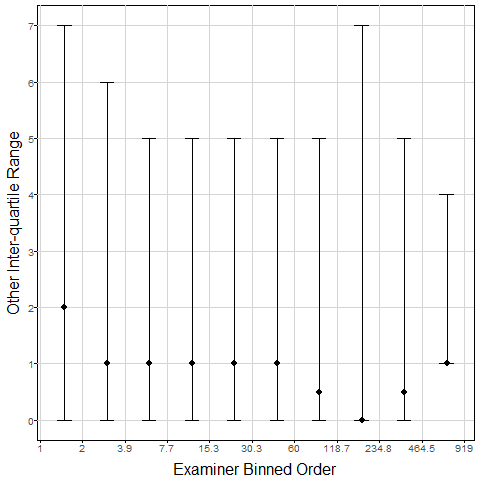
\includegraphics[width=0.9\linewidth]{Figures/MedianOtherVsExaminer}
  \caption[]{\small Median Other for Binned Examiner }
\label{fig:MedianOtherVsExaminer}
\end{subfigure}
\begin{subfigure}{.24\linewidth}
  \centering
  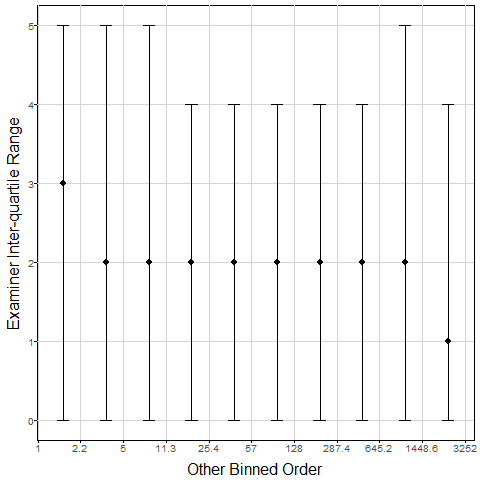
\includegraphics[width=0.9\linewidth]{Figures/MedianExaminerVsOther}
  \caption[]{\small Median examiner for binned Other}
\label{fig:MedianExaminerVsOther}
\end{subfigure}
\caption[]{Comparison of 'Other' and 'Examiner' sub-graphs degree correlation by logarithmically binning one and calculating metrics about the other (mean/median) }
\label{fig:binnedAverageComparison}
\end{figure}

\begin{table}
\caption{Correlation metrics and their P values. Pearson transformed refers to Pearson correlation conducted on log-log transformed data}
\label{tab:cor}
\centering
\begin{tabular}{l l l l}
\toprule
Statistic & Value & One-sided (Less) & Two-sided \\
\midrule
Kendall's Tau & -0.0889 & 2.2e-16 & 2.2e-16 \\
Pearson Correlation & -0.008 & 5.5e-3 & 1.1e-2 \\
Pearson transformed & -0.0378 & 2.2e-16 & 2.2e-16  \\
Spearman's rho & -0.1243 & 2.2e-16 & 2.2e-16 \\
\bottomrule\\
\end{tabular}
\end{table}

%----------------------------------------------------------------------------------------
%	SECTION 2
%----------------------------------------------------------------------------------------

\subsection{Fitting Distributions} \label{section: Fitting Distributions}

As in section \ref{Degree Distribution} four different functional forms are fitted to the cumulative degree distribution using maximum likelihood estimators while optimising $x_{min}$ to minimise the Kolmogorov-Smirnov statistic as a measure of goodness-of-fit. Here the year 2002 is used as a year present in the Valverde analysis which has Examiner and Other networks analysable. A bootstrapping method using 2500 samples to compute a P value to an approximate accuracy of 0.1 is used using the same methods as previously. This method is conducted on a sample of 10000 observations due to the performance limitations of the method. Due to this sample being a relatively small subset of the data results from this are taken with caution. A log-likelihood ratio test is also used to compare distributions, this uses all the available data rather than a sample but first refits the distributions so that both fits share the same $x_{min}$, this is done by setting the $x_{min}$ as the greater of the two previous fits, as it is more conservative, before solving for the other parameter(s) by maximising the likelihood function. 

\begin{figure}
\centering
  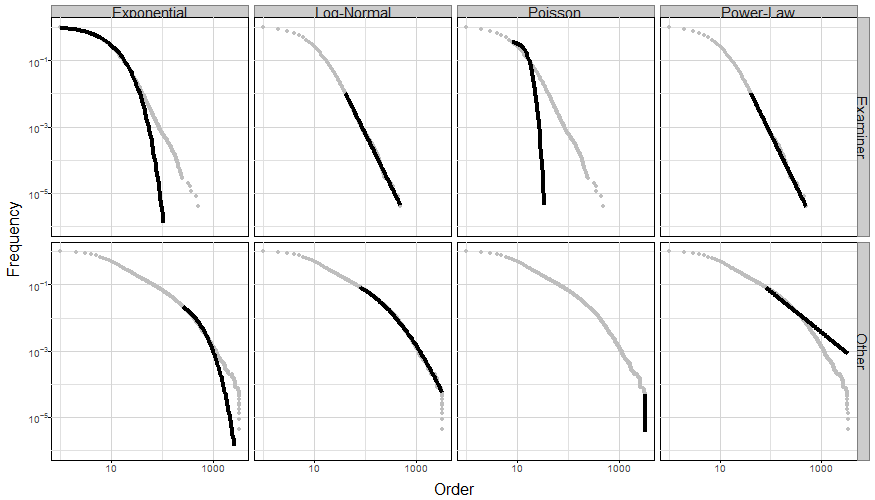
\includegraphics[width=0.7\linewidth]{Figures/ExaminerOtherDistributionFit}
  \caption[Fitting Degree Distribution for "Examiner" and "Other" sub-graphs]{Fitted 2002 degree distributions for "Other" and "Examiner" sub-graphs using Maximum Likelihood for discrete distributions: Poisson, Exponential, Log-normal, Power-law.}
\label{fig:ExaminerOtherDistributionFit}
\end{figure}

\begin{table}
\caption{P values fitting distributions to the degree distribution obtained through bootstrapping method on a n = 10000 sample of the data}
\label{tab:distributionsColouredP}
\centering
\begin{tabular}{l l l l l}
\toprule
CitedBy & Power-Law & Log-Normal & Poisson & Exponential \\
\midrule
Examiner & 0.177 & 0.024 & 0.000 & 0.090 \\
Other & 0.343 & 0.327 & 0.037 & 0.000 \\
\bottomrule\\
\end{tabular}
\end{table}

\begin{table}
\caption{P values for likelihood data is power law distributed in comparison to log-normal using likelihood ratio test}
\label{tab:distributionsColouredP2}
\centering
\begin{tabular}{l l l l}
\toprule
CitedBy & Log Likelihood Ratio & P: One sided & P: Two Sided \\
\midrule
Examiner & 0.352 & 0.637 & 0.725 \\
Other & -14.78 &9.75e-50 & 1.95e-49 \\
\bottomrule\\
\end{tabular}
\end{table}

As in section \ref{Degree Distribution} a P value of less than 0.1 is taken as a rule of thumb to be discounted. Here all the P values are significantly lower than before and none of the Poisson or Exponential distributions get a significant result. While the Other network shows very similar P values for Power-Law and Log-Normal the Examiner network has very low values for the Log-Normal, lower than the Exponential and lower than the threshold for significance. When using the log-likelihood ratio test to compare distributions however the Examiner gives a high 2 sided P value. The two sided test indicates the probability that the data comes from both distributions i.e. that they are both good fits to the data and can't be analytically distinguished. This is in conflict with the bootstrapping results although as previously stated the small sample size makes these results fairly unreliable. The Other class however completely has vanishingly small p values for a power law suggesting that this can be discounted and a log-normal is the better fit. 

When comparing these results to the time varying ones from section \ref{Degree Distribution} the Examiner sub-network shows similar results to the 1984 analysis whereas the Other sub-network shows similar results to the more recent (2002/2012) analysis. This helps to support the idea that the relative dominance of the applicant citations is a structural change in the network. 

%----------------------------------------------------------------------------------------
%	SECTION 2
%----------------------------------------------------------------------------------------

\subsection{Patent growth over time}

In order to try to identify further the changes in structure of the network over time, we look at how the parameters of power-law and log-normal fits have changed over time. Each year is fitted with a power-law distribution, maximising the likelihood while searching over a range of $x_{min}$ values as before. After the year 2001 this is also computed separately for the Examiner and Other sub-network respectively. This process is repeated for log-normal distribution. While the power-law only has one parameter, $\alpha$, the log-normal has two, $\mu$ and $\sigma$. 

Figure \ref{fig:paramsOverTime_pl} shows the power-law parameters as they change over time. Note the Other distribution has its exponent changing over a wide range in a noisy manner. The power-law is a poor fit for this distribution and so over different years the power-law is fitting to different parts of the curve by varying $x_{min}$ by large amounts, this is demonstrated in figure \ref{fig:plFits}. When $x_{min}$ is relatively small the parameter shadows that of the total as you would expect. As seen earlier the Examiner has smaller exponents however for this data over this time period it is hard to identify any diverging trends between the two if any exist. 

The parameters for the log-normal, are more insightful \ref{fig:logNormalParams}. The total has a tight cluster of years with a few outliers, the Other occupies only this cluster while the Examiner has points both in the cluster and the outlier region. Zooming in on the cluster there is a similar story where the total occupying a cluster but also some space away from that tight cluster. The cluster are the fits from the last 10 years and are clearly separable from before this point. The other occupies a parameter space very close to this cluster where the Examiner occupies a parameter space which is representative of the Total before the last 10 years. This further supports the hypothesis that the network was once much more strongly influenced by the examiner sub-network as the structure of the network now when fitted with the log-normal distribution is similar to the whole network fitted with this distribution 10-20 years ago.  

\begin{figure}
\centering
  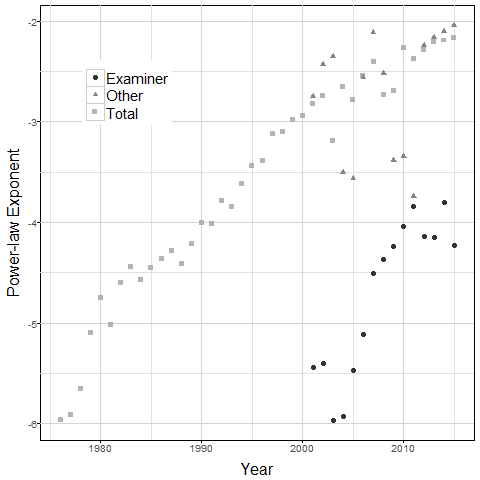
\includegraphics[width=0.7\linewidth]{Figures/paramsOverTime_pl}
  \caption[Variation of Power-Law exponent over time]{Variation in the exponent of the Power-Law fit for degree distribution from 1976:2015, where available "Examiner" and "Other" sub-graphs are also computed}
\label{fig:paramsOverTime_pl}
\end{figure}

\begin{figure}
\centering
\begin{subfigure}{.5\textwidth}
  \centering
  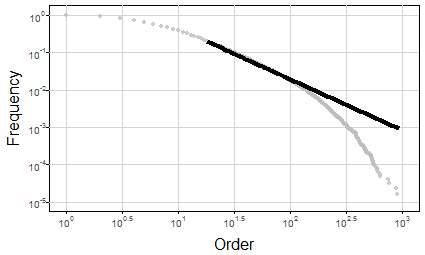
\includegraphics[width=0.9\linewidth]{Figures/plFit2003}
 \caption[]{\small Power-Law fit for "Other" sub-graph in 2003}
\label{fig:plFit2003}
\end{subfigure}%
\begin{subfigure}{.5\textwidth}
  \centering
  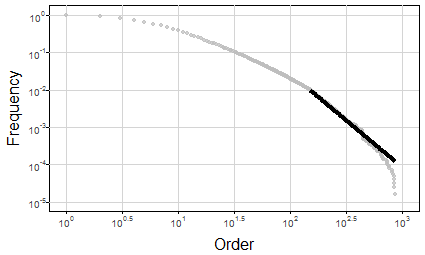
\includegraphics[width=0.9\linewidth]{Figures/plFit2004}
  \caption[]{\small Power-Law fit for "Other" sub-graph in 2004}
\label{fig:plFit2004}
\end{subfigure}
\caption[Power-law fitting to different parts of the curve for the "Other" sub-graph]{}
\label{fig:plFits}
\end{figure}

\begin{figure}
\centering
\begin{subfigure}{.7\textwidth}
  \centering
  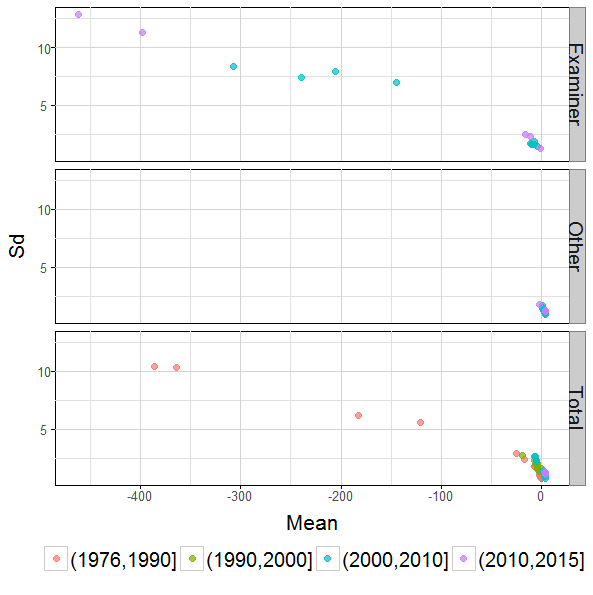
\includegraphics[width=0.9\linewidth]{Figures/logNormalParams}
 \caption[]{\small Overview}
\label{fig:logNormalParams}
\end{subfigure}%

\begin{subfigure}{.7\textwidth}
  \centering
  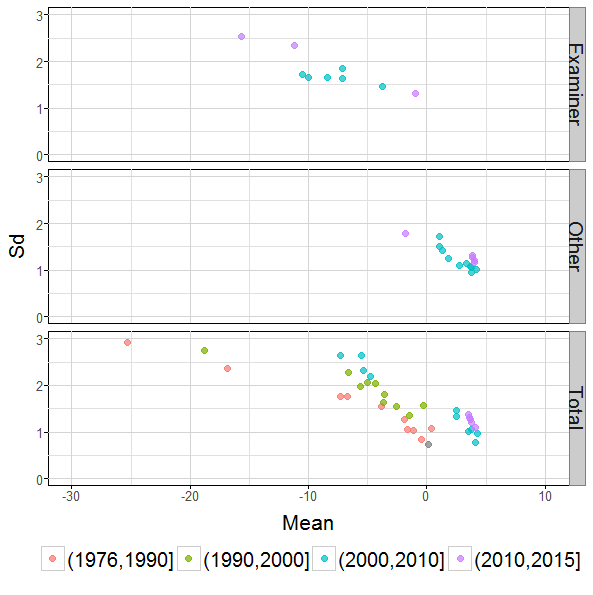
\includegraphics[width=0.9\linewidth]{Figures/logNormalParams_zoomed}
  \caption[]{\small Zoomed in on cluster}
\label{fig:logNormalParams_zoomed}
\end{subfigure}
\caption[Variation of Log-normal parameters over time]{Variation in the mean and standard deviation of log-normal fits each year 1976 to 2015 for cited by "Examiner", cited by "Other" and combined. Colour representing the decade}
\label{fig:logNormalParamPlots}
\end{figure}